\part{Approcci di risoluzione}

\begin{frame}
	\partpage
	\centering
\end{frame}

\begin{frame}
	\frametitle{Ricerca esaustiva}
	Elenco tutti i possibili percorsi 

	Complessità
	\begin{itemize}
		\item Tempo: $O(|V|^q)$ $\rightarrow$ Color Coding $\rightarrow$ $O(2^q\ |V|)$
		\item Spazio: $O(|\Sigma|^q\ q)$ $\rightarrow$ Sampling $\rightarrow$ $O(rq)$
	\end{itemize}
\end{frame}

\begin{frame}
	\frametitle{Color Coding}
	\centering


		\begin{minipage}{.45\textwidth}
			\centering
			Coloriamo casualmente il grafo con $q$ colori e ci limitiamo ai path colorful 
			(percorsi con colori non ripetuti)
			\medskip
			
			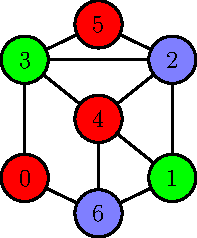
\includegraphics[width=0.5\textwidth]{images/8_cc_graph}
			
			\small
			\medskip
			
			Il numero dei path è esponenzialmente ridotto di un fattore $q! / q^q \simeq e^{-q}$\\
			 
			Per $q=3$ solo il $\sim22.22\%$\\
			Per $q=6$ solo il $\sim1.5\%$\phantom{$22$}
		\end{minipage}\hfill
		\begin{minipage}{.45\textwidth}
			\centering
			$q!$ colorazioni accettabili\\
			$q^q$ possibili colorazioni
			
			\medskip
			
			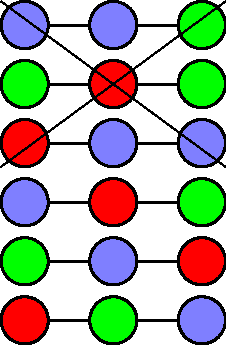
\includegraphics[width=0.5\textwidth]{images/8_cc_list}
			
			Esempi di possibili path
			\hfill
		\end{minipage}\hfill

\end{frame}

\begin{frame}
	\frametitle{Sampling}
	\centering
\end{frame}

\begin{frame}
	\frametitle{F-Count}
	\centering
\end{frame}

\begin{frame}
	\frametitle{F-Samp}
	\centering
\end{frame}

%\begin{frame}
%	\frametitle{Baseline}
%	\centering
%\end{frame}
